\documentclass[oneside]{book}
\usepackage{ctex}
\usepackage{amsmath, amsthm, amssymb, amsfonts}
\usepackage{thmtools}
\usepackage{graphicx}
\usepackage{setspace}
\usepackage{geometry}
\usepackage{float}
\usepackage{hyperref}
\usepackage[utf8]{inputenc}
\usepackage[english]{babel}
\usepackage{framed}
\usepackage[dvipsnames]{xcolor}
\usepackage{environ}
\usepackage{tcolorbox}
\usepackage{enumerate}
\usepackage{mathrsfs}
\newcommand*{\dif}{\mathop{}\!\mathrm{d}}
\tcbuselibrary{theorems,skins,breakable}


\setstretch{1.2}
\geometry{
	textheight=9in,
	textwidth=5.5in,
	top=1in,
	headheight=12pt,
	headsep=25pt,
	footskip=30pt
}

% Variables
\def\notetitle{An Introduction to Partial Differential Equations}
\def\noteauthor{
	\textbf{Professor Jun Geng} \\ 
	{\LaTeX} by Yixin Wang\\
	Lanzhou University}
\def\notedate{Semester 1}

% The theorem system and user-defined commands
% Theorem System
% The following boxes are provided:
%   Definition:     \defn 
%   Theorem:        \thm 
%   Lemma:          \lem
%   Corollary:      \cor
%   Proposition:    \prop   
%   Claim:          \clm
%   Fact:           \fact
%   Proof:          \pf
%   Example:        \ex
%   Remark:         \rmk (sentence), \rmkb (block)
% Suffix
%   r:              Allow Theorem/Definition to be referenced, e.g. thmr
%   p:              Add a short proof block for Lemma, Corollary, Proposition or Claim, e.g. lemp
%                   For theorems, use \pf for proof blocks

% Definition
\newtcbtheorem[number within=section]{mydefinition}{Definition}
{
	enhanced,
	frame hidden,
	titlerule=0mm,
	toptitle=1mm,
	bottomtitle=1mm,
	fonttitle=\bfseries\large,
	coltitle=black,
	colbacktitle=green!20!white,
	colback=green!10!white,
}{defn}

\NewDocumentCommand{\defn}{m+m}{
	\begin{mydefinition}{#1}{}
		#2
	\end{mydefinition}
}

\NewDocumentCommand{\defnr}{mm+m}{
	\begin{mydefinition}{#1}{#2}
		#3
	\end{mydefinition}
}

% Theorem
\newtcbtheorem[use counter from=mydefinition]{mytheorem}{Theorem}
{
	enhanced,
	frame hidden,
	titlerule=0mm,
	toptitle=1mm,
	bottomtitle=1mm,
	fonttitle=\bfseries\large,
	coltitle=black,
	colbacktitle=cyan!20!white,
	colback=cyan!10!white,
}{thm}

\NewDocumentCommand{\thm}{m+m}{
	\begin{mytheorem}{#1}{}
		#2
	\end{mytheorem}
}

\NewDocumentCommand{\thmr}{mm+m}{
	\begin{mytheorem}{#1}{#2}
		#3
	\end{mytheorem}
}

% Lemma
\newtcbtheorem[use counter from=mydefinition]{mylemma}{Lemma}
{
	enhanced,
	frame hidden,
	titlerule=0mm,
	toptitle=1mm,
	bottomtitle=1mm,
	fonttitle=\bfseries\large,
	coltitle=black,
	colbacktitle=violet!20!white,
	colback=violet!10!white,
}{lem}

\NewDocumentCommand{\lem}{m+m}{
	\begin{mylemma}{#1}{}
		#2
	\end{mylemma}
}

\newenvironment{lempf}{
	{\noindent{\it \textbf{Proof for Lemma}}}
	\tcolorbox[blanker,breakable,left=5mm,parbox=false,
	before upper={\parindent15pt},
	after skip=10pt,
	borderline west={1mm}{0pt}{violet!20!white}]
}{
	\textcolor{violet!20!white}{\hbox{}\nobreak\hfill$\blacksquare$} 
	\endtcolorbox
}

\NewDocumentCommand{\lemp}{m+m+m}{
	\begin{mylemma}{#1}{}
		#2
	\end{mylemma}
	
	\begin{lempf}
		#3
	\end{lempf}
}

% Corollary
\newtcbtheorem[use counter from=mydefinition]{mycorollary}{Corollary}
{
	enhanced,
	frame hidden,
	titlerule=0mm,
	toptitle=1mm,
	bottomtitle=1mm,
	fonttitle=\bfseries\large,
	coltitle=black,
	colbacktitle=orange!20!white,
	colback=orange!10!white,
}{cor}

\NewDocumentCommand{\cor}{+m}{
	\begin{mycorollary}{}{}
		#1
	\end{mycorollary}
}

\newenvironment{corpf}{
	{\noindent{\it \textbf{Proof for Corollary.}}}
	\tcolorbox[blanker,breakable,left=5mm,parbox=false,
	before upper={\parindent15pt},
	after skip=10pt,
	borderline west={1mm}{0pt}{orange!20!white}]
}{
	\textcolor{orange!20!white}{\hbox{}\nobreak\hfill$\blacksquare$} 
	\endtcolorbox
}

\NewDocumentCommand{\corp}{m+m+m}{
	\begin{mycorollary}{}{}
		#1
	\end{mycorollary}
	
	\begin{corpf}
		#2
	\end{corpf}
}

% Proposition
\newtcbtheorem[use counter from=mydefinition]{myproposition}{Proposition}
{
	enhanced,
	frame hidden,
	titlerule=0mm,
	toptitle=1mm,
	bottomtitle=1mm,
	fonttitle=\bfseries\large,
	coltitle=black,
	colbacktitle=yellow!30!white,
	colback=yellow!20!white,
}{prop}

\NewDocumentCommand{\prop}{+m}{
	\begin{myproposition}{}{}
		#1
	\end{myproposition}
}

\newenvironment{proppf}{
	{\noindent{\it \textbf{Proof for Proposition.}}}
	\tcolorbox[blanker,breakable,left=5mm,parbox=false,
	before upper={\parindent15pt},
	after skip=10pt,
	borderline west={1mm}{0pt}{yellow!30!white}]
}{
	\textcolor{yellow!30!white}{\hbox{}\nobreak\hfill$\blacksquare$} 
	\endtcolorbox
}

\NewDocumentCommand{\propp}{+m+m}{
	\begin{myproposition}{}{}
		#1
	\end{myproposition}
	
	\begin{proppf}
		#2
	\end{proppf}
}

% Claim
\newtcbtheorem[use counter from=mydefinition]{myclaim}{Claim}
{
	enhanced,
	frame hidden,
	titlerule=0mm,
	toptitle=1mm,
	bottomtitle=1mm,
	fonttitle=\bfseries\large,
	coltitle=black,
	colbacktitle=pink!30!white,
	colback=pink!20!white,
}{clm}


\NewDocumentCommand{\clm}{m+m}{
	\begin{myclaim*}{#1}{}
		#2
	\end{myclaim*}
}

\newenvironment{clmpf}{
	{\noindent{\it \textbf{Proof for Claim.}}}
	\tcolorbox[blanker,breakable,left=5mm,parbox=false,
	before upper={\parindent15pt},
	after skip=10pt,
	borderline west={1mm}{0pt}{pink!30!white}]
}{
	\textcolor{pink!30!white}{\hbox{}\nobreak\hfill$\blacksquare$} 
	\endtcolorbox
}

\NewDocumentCommand{\clmp}{m+m+m}{
	\begin{myclaim*}{#1}{}
		#2
	\end{myclaim*}
	
	\begin{clmpf}
		#3
	\end{clmpf}
}

% Fact
\newtcbtheorem[use counter from=mydefinition]{myfact}{Fact}
{
	enhanced,
	frame hidden,
	titlerule=0mm,
	toptitle=1mm,
	bottomtitle=1mm,
	fonttitle=\bfseries\large,
	coltitle=black,
	colbacktitle=purple!20!white,
	colback=purple!10!white,
}{fact}

\NewDocumentCommand{\fact}{+m}{
	\begin{myfact}{}{}
		#1
	\end{myfact}
}


% Proof
\NewDocumentCommand{\pf}{+m}{
	\begin{proof}
		[\noindent\textbf{Proof.}]
		#1
	\end{proof}
}

% Example
\newenvironment{example}{%
	\par
	\vspace{5pt}
	\begin{minipage}{\textwidth}
		\noindent\textbf{Example.}
		\tcolorbox[blanker,breakable,left=5mm,parbox=false,
		before upper={\parindent15pt},
		after skip=10pt,
		borderline west={1mm}{0pt}{cyan!10!white}]
	}{%
		\endtcolorbox
	\end{minipage}
	\vspace{5pt}
}

\NewDocumentCommand{\ex}{+m}{
	\begin{example}
		#1
	\end{example}
}


% Remark
\NewDocumentCommand{\rmk}{+m}{
	{\it \color{blue!50!white}#1}
}

\newenvironment{remark}{
	\par
	\vspace{5pt}
	\begin{minipage}{\textwidth}
		{\par\noindent{\textbf{Remark.}}}
		\tcolorbox[blanker,breakable,left=5mm,
		before skip=10pt,after skip=10pt,
		borderline west={1mm}{0pt}{cyan!10!white}]
	}{
		\endtcolorbox
	\end{minipage}
	\vspace{5pt}
}

\NewDocumentCommand{\rmkb}{+m}{
	\begin{remark}
		#1
	\end{remark}
}


\newcommand{\lcm}{\operatorname{lcm}}



% ------------------------------------------------------------------------------

\begin{document}
	\title{\textbf{
			\LARGE{\notetitle} \vspace*{10\baselineskip}}
	}
	\author{\noteauthor}
	\date{\notedate}
	
	\maketitle
	\newpage
	
	\tableofcontents
	\newpage
	
	% ------------------------------------------------------------------------------
	
	\chapter{Preliminaries}
	\section{Notations}
		\begin{itemize}
			\item[(i)] \( \mathbb{R}^n = n \)-dimensional real Euclidean space, \( \mathbb{R} = \mathbb{R}^1 \). \\
			\( S^{n-1} = \partial B(0, 1) = (n-1)\)-dimensional unit sphere in \( \mathbb{R}^n \).
			
			\item[(ii)] \( e_i = (0, \dots, 0, 1, 0, \dots, 0) \) = \( i \)th standard coordinate vector.
			
			\item[(iii)] A typical point in \( \mathbb{R}^n \) is \( x = (x_1, \dots, x_n) \). \\
			We will also, depending upon the context, regard \( x \) as a row or as a column vector.
			
			\item[(iv)] \( \mathbb{R}^n_+ = \{ x = (x_1, \dots, x_n) \in \mathbb{R}^n \mid x_n > 0 \} \) = open upper half-space. \\
			\( \mathbb{R}_+ = \{ x \in \mathbb{R} \mid x > 0 \} \).
			
			\item[(v)] A point in \( \mathbb{R}^{n+1} \) will often be denoted as \( (x, t) = (x_1, \dots, x_n, t) \), and we usually interpret \( t = x_{n+1} \) = time. \\
			A point \( x \in \mathbb{R}^n \) will sometimes be written \( x = (x', x_n) \) for \( x' = (x_1, \dots, x_{n-1}) \in \mathbb{R}^{n-1} \).
			
			\item[(vi)] \( U, V, \) and \( W \) usually denote open subsets of \( \mathbb{R}^n \). We write
			\[
			V \subset\subset U
			\]
			if \( V \subset \overline{V} \subset U \) and \( \overline{V} \) is compact, and say \( V \) is \textit{compactly contained in} \( U \).
			
			\item[(vii)] \( \partial U \) = boundary of \( U \), \( \overline{U} = U \cup \partial U \) = closure of \( U \).
			
			\item[(viii)] \( U_T = U \times (0, T] \).
			
			\item[(ix)] \( \Gamma_T = \partial U_T - U_T = \) parabolic boundary of \( U_T \).
			
			\item[(x)] \( B(x, r) = \{ y \in \mathbb{R}^n \mid |x - y| \leq r \} \) = closed ball in \( \mathbb{R}^n \) with center \( x \) and radius \( r > 0 \).
			
			\item[(xi)] \( \alpha(n) \) = volume of unit ball \( B(0, 1) \) in \( \mathbb{R}^n \):
			\[
			\alpha(n) = \frac{\pi^{n/2}}{\Gamma\left(\frac{n}{2} + 1\right)}.
			\]
			\( n\alpha(n) \) = surface area of unit sphere \( \partial B(0, 1) \) in \( \mathbb{R}^n \).
		\end{itemize}
	\ex{\begin{align*}
			\int_{\mathbb{R}} e^{-x^2} \, dx &= \sqrt{\pi}. \\
			\int_{\mathbb{R}^n} e^{-|x|^2} \, dx &= \int_{-\infty}^\infty \int_{-\infty}^\infty \dots \int_{-\infty}^\infty e^{-x_1^2 - x_2^2 - \dots - x_n^2} \, dx_1 dx_2 \dots dx_n \\
			&= \pi^{n/2}.
		\end{align*}
		
		Applying Polar Coordinate,
		\begin{align*}
			\int_0^\infty r^{n-1} \int_{\partial B(0,1)} e^{-r^2} \, d\sigma \, dr &= \int_{\partial B(0,1)} d\sigma \int_0^\infty r^{n-1} e^{-r^2} \, dr \\
			&= \omega_{n-1} \int_0^\infty r^{n-1} e^{-r^2} \, dr \\
			&= \omega_{n-1} \cdot \frac{1}{2} \Gamma\left(\frac{n}{2}\right).
		\end{align*}
		\begin{align*}
			\alpha(n) = |B(0,1)| &= \int_{B(0,1)} 1 \, dx \\
			&= \int_0^1 \int_{\partial B(0,1)} r^{n-1} \, d\sigma \, dr \\
			&= \omega_{n-1} \int_0^1 r^{n-1} \, dr \\
			&= \frac{1}{n} \omega_{n-1}\\
		\end{align*}
	}
	
	\section{Calculus}
	\thmr{Gauss-Green Theorem}{GGT}{\begin{itemize}
			\item[(i)] Suppose \( u \in C^1(\overline{U}) \). Then
			
			\[ 	\int_U u_{x_i} \, dx = \int_{\partial U} u \nu^i \, dS \quad (i = 1, \dots, n). \]
			
			\item[(ii)] We have
		\[ 	
				\int_U \operatorname{div} \mathbf{u} \, dx = \int_{\partial U} \mathbf{u} \cdot \nu \, dS
			 \]
			for each vector field \( \mathbf{u} \in C^1(\overline{U}; \mathbb{R}^n) \).
		\end{itemize}
		
	}
	Assertion (ii), also called the \textit{Divergence Theorem}, follows from (i) applied to each component of \(\mathbf{u} = (u^1, \dots, u^n)\).
	\thmr{Integration by parts formula}{intbyparts}{
		Let \( u, v \in C^1(\overline{U}) \). Then
		\[    \int_U u_{x_i} v \, dx = -\int_U uv_{x_i} \, dx + \int_{\partial U} uv\nu^i \, dS \quad (i = 1, \dots, n).    \]
	}
	
	\pf{
		Apply Gauss-Green Theorem to \( uv \).
	}
	
	\thmr{Green's formulas}{greens}{
		Let \( u, v \in C^2(\overline{U}) \). Then
		\begin{itemize}
			\item[(i)] \[
			\int_U \Delta u \, dx = \int_{\partial U} \frac{\partial u}{\partial \nu} \, dS,
			\]
			\item[(ii)] \[
			\int_U Dv \cdot Du \, dx = -\int_U u \Delta v \, dx + \int_{\partial U} \frac{\partial v}{\partial \nu}u \, dS,
			\]
			\item[(iii)] \[
			\int_U u \Delta v - v \Delta u \, dx = \int_{\partial U} u \frac{\partial v}{\partial \nu} - v \frac{\partial u}{\partial \nu} \, dS.
			\]
		\end{itemize}
	}
	
	\pf{
		Using the \textit{Integration by parts formula} with \( u_{x_{i}} \) in place of \( u \) and \( v \equiv 1 \), we see
		\[
		\int_U u_{x_i x_i} \, dx = \int_{\partial U} u_{x_i} \nu^i \, dS.
		\]
		Summing over \( i = 1, \dots, n \) establishes (i).
		
		To derive (ii), we employ the \textit{Integration by parts formula} with \( v_{x_i} \) replacing \( v \). Write (ii) with \( u \) and \( v \) interchanged and then subtract to obtain (iii).
	}
	\rmkb{$D u\cdot\nu = \dfrac{\partial u}{\partial\nu}$}
	
	\thmr{Polar coordinates}{polar}{
		\begin{itemize}
			\item[(i)] Let \( f : \mathbb{R}^n \to \mathbb{R} \) be continuous and summable. Then
			\[
			\int_{\mathbb{R}^n} f \, dx = \int_0^\infty \left( \int_{\partial B(x_0, r)} f \, dS \right) dr
			\]
			for each point \( x_0 \in \mathbb{R}^n \).
			\item[(ii)] In particular,
			\[
			\frac{d}{dr} \left( \int_{B(x_0, r)} f \, dx \right) = \int_{\partial B(x_0, r)} f \, dS
			\]
			for each \( r > 0 \).
		\end{itemize}
	}
	\section{Measure Theory}
	\thmr{Dominated Convergence Theorem}{domconv}{
		Assume the functions \( \{f_k\}_{k=1}^\infty \) are integrable and
		\[
		f_k \to f \quad \text{a.e.}
		\]
		Suppose also
		\[
		|f_k| \leq g \quad \text{a.e.},
		\]
		for some summable function \( g \). Then
		\[
		\int_{\mathbb{R}^n} f_k \, dx \to \int_{\mathbb{R}^n} f \, dx.
		\]
	}
	\pf{See notes for Real Analysis.}
	
	\thmr{Lebesgue's Differentiation Theorem}{lebdiff}{
		Let \( f : \mathbb{R}^n \to \mathbb{R} \) be locally summable.
		\begin{itemize}
			\item[(i)] Then for a.e. point \( x_0 \in \mathbb{R}^n \),
			\[
			\frac{1}{|B(x_0, r)|} \int_{B(x_0, r)} f \, dx \to f(x_0) \quad \text{as } r \to 0.
			\]
			\item[(ii)] In fact, for a.e. point \( x_0 \in \mathbb{R}^n \),
			\[
			\frac{1}{|B(x_0, r)|} \int_{B(x_0, r)} |f(x) - f(x_0)| \, dx \to 0 \quad \text{as } r \to 0.
			\]
		\end{itemize}
	}
	
	\chapter{Four Important Linear Partial Differential Equations}	
	\section{Laplace Equation}
	Among the most important of all partial differential equations are undoubtedly \textit{Laplace's equation}
	\[ 
		\Delta u = 0
	 \]
	and \textit{Poisson's equation}
	\[ 
		-\Delta u = f.
	 \]
	First of all we study the properties of \textbf{harmonic} functions.
	\defn{Harmonic Function}{
		A \( C^2 \) function \( u \) satisfying \( \Delta u = 0 \) is called a \textit{harmonic function}.
	}
	\subsection{Mean-Value Formulas}
	\thmr{Mean-value formulas for Laplace's equation}{meanval}{
		If \( u \in C^2(U) \) is harmonic, then
		\[
		u(x) = \frac{1}{|\partial B(x,r)|} \int_{\partial B(x,r)} u \, d\sigma = \frac{1}{|B(x,r)|} \int_{B(x,r)} u \, dy
		\]
		for each ball \( B(x, r) \subset U \).
	}
	\pf{
		Set
		\[
		\varphi(r) = \frac{1}{|\partial B(x,r)|} \int_{\partial B(x,r)} u(y) \, d\sigma(y),
		\]
		where
		\[
		|\partial B(x,r)| = n\alpha(n) r^{n-1}, \quad \text{and } \alpha(n) = \frac{\pi^{n/2}}{\Gamma\left(\frac{n}{2} + 1\right)}.
		\]
		
		By a change of variables \( y = x + rz \), we have
		\[
		\varphi(r) = \frac{r^{n-1}}{n\alpha(n) r^{n-1}} \int_{\partial B(0,1)} u(x + rz) \, d\sigma(z).
		\]
		
		Then,
		\[
		\varphi'(r) = \frac{1}{n\alpha(n) } \int_{\partial B(0,1)} \nabla u(x + rz) \cdot z \, d\sigma(z).
		\]
		
		By the divergence theorem:
		\[
		\int_{\partial B(x,r)} \frac{\partial u}{\partial \nu} \, d\sigma = \int_{B(x,r)} \Delta u \, dy.
		\]
		
		We have\[ \begin{aligned}
			\varphi^{\prime}(r) &= \frac{1}{n\alpha(n) } \int_{\partial B(0,1)} \nabla u(x + rz) \cdot \dfrac{y-x}{r} \, d\sigma(z) \\
			&= \frac{1}{n\alpha(n)r^{n-1} } \int_{\partial B(x,r)} \nabla u(y) \cdot \nu \, d\sigma(y)\\
			&= \frac{1}{n\alpha(n)r^{n-1} } \int_{\partial B(x,r)} \dfrac{\partial u (y)}{\partial\nu}  \, d\sigma(y)\\
			&= \frac{1}{n\alpha(n)r^{n-1} } \int_{ B(x,r)} \Delta u (y)  \, dy\\
			&= \dfrac{r}{n}\cdot\dfrac{1}{|B(x,r)|}\int_{ B(x,r)} \Delta u (y)  \, dy
		\end{aligned} \]
		
		Since \( u \) is harmonic (\( \Delta u = 0 \)), we conclude that \( \varphi'(r) = 0 \), which implies that \( \varphi(r) \) is constant.
		
		By the Lebesgue Differentiation Theorem
		\[
		\varphi(r) =\lim_{t \to 0} \frac{1}{|\partial B(x,t)|} \int_{\partial B(x,t)} u \, d\sigma = u(x)
		\]
		
		By employing polar coordinates, we have
		\[
		\int_{B(x,r)} u \, dy = \int_0^r \int_{\partial B(x,s)} u \, d\sigma \, ds
		\]
		and
		\[
		\int_{B(x,r)} u \, dy = n\alpha(n) \int_0^r s^{n-1} u(x) \, ds.
		\]
		
		Finally,
		\[
		u(x) = \frac{1}{|B(x,r)|} \int_{B(x,r)} u \, dy.
		\]
	}
	
	\thmr{Converse to mean-value property}{meanvalconv}{
		If \( u \in C^2(U) \) satisfies
		\[
		u(x) = \frac{1}{|\partial B(x,r)|} \int_{\partial B(x,r)} u \, dS
		\]
		for each ball \( B(x,r) \subset U \), then \( u \) is harmonic.
	}
	\pf{
		Suppose not. WLOG, there exists a ball \( B(x, r) \subset U \), such that \( \Delta u > 0 \) in \( B(x, r) \).
		
		Define
		\[
		\varphi(r) = \dfrac{1}{|B(x,r)|}\int_{\partial B(x,r)} u \, d\sigma.
		\]
		
		Then
		\[
		\varphi'(r) = \dfrac{r}{n}\cdot\dfrac{1}{|B(x,r)|}\int_{ B(x,r)} \Delta u (y)  \, dy > 0.
		\]
		
		However, since \( \varphi(r) \) is a constant, \( \varphi'(r) = 0 \), which is a contradiction (as \( \Delta u > 0 \)).
		Therefore, \( u \) must be harmonic.
	}
	\subsection{Maximum Principle}
		\thm{Strong maximum principle}{
			Suppose \( u \in C^2(U) \cap C(\overline{U}) \) is harmonic within \( U \).
			\begin{itemize}
				\item[(i)] Then 
				\[
				\max_{\overline{U}} u = \max_{\partial U} u.
				\]
				\item[(ii)] Furthermore, if \( U \) is connected and there exists a point \( x_0 \in U \) such that 
				\[
				u(x_0) = \max_{\overline{U}} u,
				\]
				then \( u \) is constant within \( U \).
			\end{itemize}
			Assertion (i) is the maximum principle for Laplace's equation and (ii) is the strong maximum principle. Replacing \( u \) by \( -u \), we recover also similar assertions with "min" replacing "max".
		}
		
		\pf{
			Suppose \( \exists x_0 \in U \) such that \( u(x_0) = \max_{\overline{U}} u := M \).
			
			Then for \( 0 < r < \delta(x_0) = \operatorname{dist}(x_0, \partial  U) \), the mean value property implies that
			\[
			u(x_0) = \frac{1}{|B(x_0, r)|} \int_{B(x_0, r)} u(x) \, dx \leq M.
			\]
			
			Since \( u(x_0) = M \), equality holds iff \( u(x) = M \) for all \( x \in B(x_0, r) \).
			
			Repeating this argument, we see that \( u(y) = M \) for all \( y \in B(x_0, r) \).
			
			Hence the set \( \{ x \in U \mid u(x) = M \} \) is both open and relatively closed in \( U \), and thus equals \( U \) if \( U \) is connected.
		}
		Before we learn the weak maximum principle, we first introduce the following definition:
		\defn{Subharmonic and Superharmonic Functions}{
			Let \( u \) be a \( C^2 \) function in \( U \). Then \( u \) is a subharmonic (superharmonic) function in \( U \) if \( \Delta u \geq 0 \) (\( \Delta u \leq 0 \)).
		}
		Subharmonic and superharmonic functions both have maximum principle, we only show one of it.
		\thm{Maximum Principle for Subharmonic Functions}{
			Let \( U \) be a bounded domain in \( \mathbb{R}^n \) and \( u \in C^2(U) \cap C(\overline{U}) \) be subharmonic in \( U \). Then \( u \) attains its maximum in \( \overline{U} \), i.e.,
			\[
			\max_{\overline{U}} u = \max_{\partial U} u.
			\]
		}
		
		\pf{
			1. First, consider \( \Delta u > 0 \) in \( U \). If \( u \) has a local maximum at a point \( x_0 \in U \), then the Hessian matrix \( \nabla^2 u(x_0) \) is negative semi-definite. Thus,
			\[
			\Delta u(x_0) = \operatorname{tr}(\nabla^2 u(x_0)) \leq 0,
			\]
			which is a contradiction.
			
			2. Now consider \( \Delta u \geq 0 \). To handle this, for any \( \varepsilon > 0 \), define
			\[
			u_\varepsilon(x) = u(x) + \varepsilon |x|^2.
			\]
			Then,
			\[
			\Delta u_\varepsilon(x) = \Delta u(x) + \Delta (\varepsilon |x|^2) = \Delta u(x) + 2n\varepsilon > 0.
			\]
			By Step 1, we have
			\[
			\max_{\overline{U}} u_\varepsilon = \max_{\partial U} u_\varepsilon.
			\]
			
			Observe that
			\[
			\max_{\overline{U}} u \leq \max_{\overline{U}} u_\varepsilon = \max_{\partial U} u_\varepsilon \leq \max_{\partial U} u + \max_{\partial U} (\varepsilon |x|^2).
			\]
			Taking \( \varepsilon \to 0 \), we conclude
			\[
			\max_{\overline{U}} u = \max_{\partial U} u.
			\]
		}
		
		\thm{Uniqueness}{
			Let \( g \in C(\partial U) \), \( f \in C(U) \). Then there exists at most one solution \( u \in C^2(U) \cap C(\overline{U}) \) of the boundary-value problem
			\[
			\begin{cases}
				-\Delta u = f & \text{in } U, \\
				u = g & \text{on } \partial U.
			\end{cases}
			\]
		}
		
		\pf{
			If \( u \) and \( \tilde{u} \) are both solutions for the boundary-value problem , apply maximum principle to the harmonic functions \( w := \pm (u - \tilde{u}) \).
		}
		\rmkb{If $U$ is unbounded, the conclusion fails.}
		
		\subsection{Regularity}
		Our main result in this section is that if $u\in C^{2}$ is harmonic, then necessarily $u\in C^{\infty}$.
		
		Let \( \Omega \subset \mathbb{R}^n \) be open. For \( \varepsilon > 0 \), denote
		\[
		\Omega_\varepsilon = \{ x \in \Omega \mid \text{dist}(x, \partial \Omega) > \varepsilon \}.
		\]
		
		\defn{Mollifier}{
			Define the mollifier as:
			\[
			\eta(x) =
			\begin{cases}
				C \exp\left(\frac{1}{ |x|^2 - 1}\right), & \text{if } |x| < 1, \\
				0, & \text{if } |x| \geq 1.
			\end{cases}
			\]
			where \( \eta \in C^\infty(\mathbb{R}^n) \) and satisfies \( \int_{\mathbb{R}^n} \eta(x) \, dx = 1 \).
			
			Let
			\[
			\eta_\varepsilon(x) = \frac{1}{\varepsilon^n} \eta\left(\frac{x}{\varepsilon}\right).
			\]
			This is called the \textit{standard mollifier}.
		}
		By definition, we know that $\eta_{\varepsilon}$ has support, and $spt(\eta_{\varepsilon})\subset B(0,\varepsilon)$.
		\defn{Mollification}{
			For a function \( f \), define its mollification as:
			\[
			f^\varepsilon = \eta_\varepsilon * f = \int_{\Omega} \eta_\varepsilon(x-y) f(y) \, dy = \int_{B(0,\varepsilon)} \eta_\varepsilon(y) f(x-y) \, dy.
			\]
		}
		\thm{Properties of molifiers}{$f^{\varepsilon}\in C^{\infty}(\Omega_{\varepsilon})$.}
		\pf{
			We can rewrite:
			\[
			f^\varepsilon(x) = \int_{\Omega} \eta_\varepsilon(y) f(x - y) \, dy = \frac{1}{\varepsilon^n} \int_{\Omega} \eta\left(\frac{y}{\varepsilon}\right) f(x - y) \, dy.
			\]
			Change variables with \( z = \frac{y}{\varepsilon} \), \( dy = \varepsilon^n dz \):
			\[
			f^\varepsilon(x) = \int_{\mathbb{R}^n} \eta(z) f(x - \varepsilon z) \, dz.
			\]
			Since \( \eta \in C^\infty \), we conclude \( f^\varepsilon \in C^\infty \).
				In fact, fix \( x \in U_\varepsilon \), \( i \in \{ 1, \dots, n \} \), and \( h \) so small that \( x + h e_i \in U_\varepsilon \). Then:
				\[
				\frac{f^\varepsilon(x + h e_i) - f^\varepsilon(x)}{h} = \frac{1}{\varepsilon^n} \int_\Omega \frac{1}{h} \left[ \eta\left(\frac{x + h e_i - y}{\varepsilon}\right) - \eta\left(\frac{x - y}{\varepsilon}\right)\right] f(y) \, dy
				\]
				\[
				= \frac{1}{\varepsilon^n} \int_V \frac{1}{h} \left[ \eta\left(\frac{x + h e_i - y}{\varepsilon}\right) - \eta\left(\frac{x - y}{\varepsilon}\right)\right] f(y) \, dy,
				\]
				for some open set \( V \subset\subset U \). As
				\[
				\frac{1}{h} \left[ \eta\left(\frac{x + h e_i - y}{\varepsilon}\right) - \eta\left(\frac{x - y}{\varepsilon}\right)\right] \to \frac{1}{\varepsilon} \eta_{x_i}\left(\frac{x - y}{\varepsilon}\right)
				\]
				uniformly on \( V \), the partial derivative \( f^\varepsilon_{x_i}(x) \) exists and equals
				\[
				f^\varepsilon_{x_i}(x) = \int_\Omega \eta_{\varepsilon, x_i}(x - y) f(y) \, dy.
				\]
				
				A similar argument shows that \( D^\alpha f^\varepsilon(x) \) exists, and
				\[
				D^\alpha f^\varepsilon(x) = \int_\Omega D^\alpha \eta_\varepsilon(x - y) f(y) \, dy, \quad (x \in U_\varepsilon),
				\]
				for each multiindex \( \alpha \). 
			
			
		}
		
		\thm{Smoothness}{
			Suppose \( u \in C^2(\Omega) \) and \( \Delta u = 0 \) in \( \Omega \). Then \( u \in C^\infty(\Omega) \).
		}
		
		\pf{
			Let \( \eta \) be the standard mollifier. Define
			\[
			u^\varepsilon(x) = \eta_\varepsilon * u = \int_{\Omega} \eta_\varepsilon(x-y) u(y) \, dy = \frac{1}{\varepsilon^n} \int_{B(x, \varepsilon)} \eta\left(\frac{x-y}{\varepsilon}\right) u(y) \, dy.
			\]
			Using polar coordinates and the mean value property:
			\[
			\begin{aligned}
				u^\varepsilon(x) &= \frac{1}{\varepsilon^n} \int_{0}^{\varepsilon}\int_{\partial B(x, r)} \eta\left(\frac{r}{\varepsilon}\right) u(y) \, d\sigma dr \\
				&= \frac{1}{\varepsilon^n} \int_{0}^{\varepsilon} \eta\left(\frac{r}{\varepsilon}\right) \frac{n\alpha(n) r^{n-1}}{n\alpha(n) r^{n-1}} \int_{\partial B(x, r)} u(y) \, d\sigma dr\\
				&=\frac{1}{\varepsilon^n} \int_{0}^{\varepsilon} \eta\left(\frac{r}{\varepsilon}\right) n\alpha(n) r^{n-1}u(x) \, dr\\
				&= u(x)\frac{1}{\varepsilon^n} \int_{0}^{\varepsilon}\int_{\partial B(x,r)} \eta\left(\frac{r}{\varepsilon}\right) \, d\sigma dr\\
				&= u(x)\int_{B(x,\varepsilon)}\dfrac{1}{\varepsilon^{n}}\eta\left(\frac{r}{\varepsilon}\right) \, dr\\
				&= u(x)\in C^{\infty}(\Omega_{\varepsilon})
			\end{aligned}
			\]
			
		}
		
		The stronger conclusion is that 
		\thm{Analyticity}{Assume $u$ is harmonic in $\Omega$, then $u$ is analytic in $\Omega$}.
		
		\subsection{Interior Estimate}
		\thm{Estimates on Derivatives (Theorem 7)}{
			Assume \( u \) is harmonic in \( U \). Then:
			\[
			|D^\alpha u(x_0)| \leq \frac{C_k}{r^{n+k}} \| u \|_{L^1(B(x_0, r))}
			\]
			for each ball \( B(x_0, r) \subset U \) and each multiindex \( \alpha \) of order \( |\alpha| = k \). 
			
			Here:
			\[
			C_0 = \frac{1}{\alpha(n)}, \quad C_k = \frac{(2^{n+1}nk)^k}{\alpha(n)}, \quad (k = 1, 2, \dots),
			\]
			where \( \alpha(n) \) is the volume of the unit ball in \( \mathbb{R}^n \).
		}
		
		\pf{
			We argue by induction on \( k \).
			
			1. For \( k = 0 \):
			\[
			\text{LHS} = u(x_0), \quad \text{RHS} = \frac{1}{\alpha(n) r^n} \int_{B(x_0, r)} u.
			\]
			Since \( u \) is harmonic, by the mean value property:
			\[
			|u(x_0)| = \frac{1}{\alpha(n) r^n} \int_{B(x_0, r)} |u| \leq \frac{1}{\alpha(n) r^n} \int_{B(x_0, r)} |u|.
			\]
			
			2. For \( k = 1 \):
			\[
			C_1 = \frac{2^n n}{\alpha(n)}.
			\]
			Observe that \( \frac{\partial u}{\partial x_i} \) is still harmonic, since \( \Delta \frac{\partial u}{\partial x_i} = \frac{\partial}{\partial x_i} (\Delta u) = 0 \).
			
			By the mean value property:
			\[
			\frac{\partial u}{\partial x_i}(x_0) = \frac{1}{\alpha(n) r^n} \int_{B(x_0, r)} \frac{\partial u}{\partial x_i}.
			\]
			
			Using the divergence theorem:
			\[
			\frac{\partial u}{\partial x_i}(x_0) = \frac{1}{\alpha(n) r^n} \int_{\partial B(x_0, r)} u \, \nu_i,
			\]
			where \( \nu_i \) is the \( i \)-th component of the outward unit normal. Then:
			\[
			\left| \frac{\partial u}{\partial x_i}(x_0) \right| \leq \frac{2^n}{\alpha(n) r^{n+1}} \| u \|_{L^1(B(x_0, r))}.
			\]
			
			Combining these inequalities, we deduce:
			\[
			| \nabla u(x_0) | \leq \frac{2^n n}{\alpha(n) r^{n+1}} \| u \|_{L^1(B(x_0, r))}.
			\]
			
			3. Inductive Step:
			Assume the estimate holds for \( k-1 \). Then for \( |\alpha| = k \), apply similar arguments using the derivatives of \( u \), the divergence theorem, and scaling properties to obtain:
			\[
			|D^\alpha u(x_0)| \leq \frac{C_k}{r^{n+k}} \| u \|_{L^1(B(x_0, r))}.
			\]
			
			Thus, the result follows by induction.
		}
		
		\chapter{Sobolev Spaces}
		\section{H{\"o}lder Spaces}
		We first discuss the simpler H{\"o}lder Spaces. Recall the definition of H{\"o}lder continuity:
		\defn{Hölder Continuity}{
			Suppose functions \( u \) satisfying 
			\[
			|u(x) - u(y)| \leq C|x - y|^\gamma \quad (x, y \in U),
			\]
			for some \( 0 < \gamma \leq 1 \) and a constant \( C \). Such a function is said to be Hölder continuous with exponent \( \gamma \).
		}
		Then we give the definition of Hölder norms.
		
		\defn{Hölder Norms}{
			\begin{itemize}
				\item[(i)] If \( u : U \to \mathbb{R} \) is bounded and continuous, we write
				\[
				\|u\|_{C(\overline{U})} := \sup_{x \in U} |u(x)|.
				\]
				\item[(ii)] The \(\gamma^{\text{th}}\)-Hölder seminorm of \( u : U \to \mathbb{R} \) is
				\[
				[u]_{C^{0,\gamma}(\overline{U})} := \sup_{x, y \in U, x \neq y} \frac{|u(x) - u(y)|}{|x - y|^\gamma}.
				\]
				The \(\gamma^{\text{th}}\)-Hölder norm is defined as
				\[
				\|u\|_{C^{0,\gamma}(\overline{U})} := \|u\|_{C(\overline{U})} + [u]_{C^{0,\gamma}(\overline{U})}.
				\]
			\end{itemize}
		}
		The general H{\"o}lder space $C^{k,\gamma}$ is defined based on it.
		\defn{H{\"o}lder Space}{The Hölder space \( C^{k,\gamma}(\overline{U}) \) consists of all functions \( u \in C^k(\overline{U}) \) for which the norm
			\[
			\|u\|_{C^{k,\gamma}(\overline{U})} := \sum_{|\alpha| \leq k} \|D^\alpha u\|_{C(\overline{U})} + \sum_{|\alpha| = k} [D^\alpha u]_{C^{0,\gamma}(\overline{U})}
			\]
			is finite.}
			
			So the space $C^{k,\gamma}(\overline{U})$ consists of those functions $u$ that are $k$-times continuously differentiable and whose $k^{\text{th}}$-partial derivatives are bounded and Hölder
			continuous with exponent $\gamma$.
			\rmkb{We may write $C^{\alpha}$ instead of $C^{0,\alpha}$ for brevity.} 
		\section{Sobolev Spaces}
			The Hölder spaces are unfortunately not often suitable settings for elementary PDE theory, as we usually cannot make good enough analytic estimates to demonstrate that the solutions we construct actually belong
			to such spaces. What are needed rather are some other kinds of spaces, containing \textbf{less smooth} functions. In practice we must strike a balance, by designing
			spaces comprising functions which have some, but not too great, smoothness
			properties.
			
			\textbf{Motivation for Definition of Weak Derivative}:
				Assume we are given a function \( u \in C^1(U) \). Then if \( \varphi \in C_c^\infty(U) \), we see from the integration by parts formula that
				\[
				\int_U u \varphi_{x_i} \, dx = -\int_U u_{x_i} \varphi \, dx \quad (i = 1, \dots, n).
				\]
				There are no boundary terms, since \( \varphi \) has compact support in \( U \) and thus vanishes near \( \partial U \). 
				
				More generally now, if \( k \) is a positive integer, \( u \in C^k(U) \), and \( \alpha = (\alpha_1, \dots, \alpha_n) \) is a multiindex of order \( |\alpha| = \alpha_1 + \dots + \alpha_n = k \), then
				\[
				\int_U u D^\alpha \varphi \, dx = (-1)^{|\alpha|} \int_U D^\alpha u \varphi \, dx.
				\]
				This equality holds since
				\[
				D^\alpha \varphi = \frac{\partial^{\alpha_1}}{\partial x_1^{\alpha_1}} \dots \frac{\partial^{\alpha_n}}{\partial x_n^{\alpha_n}} \varphi.
				\]
			
			\defn{Weak Partial Derivative}{
				Suppose \( u, v \in L_{\text{loc}}^1(U) \) and \( \alpha \) is a multiindex. We say that \( v \in L_{\text{loc}}^1(U) \) is the \(\alpha\)-weak partial derivative of \( u \), written
				\[
				D^\alpha u = v,
				\]
				provided
				\[
				\int_U u D^\alpha \varphi \, dx = (-1)^{|\alpha|} \int_U v \varphi \, dx
				\]
				for all test functions \( \varphi \in C_c^\infty(U) \).
			}
			In the sense of weak derivative, we introduce the definition of Sobolev spaces.
			\defn{Sobolev Space}{
				The Sobolev space \( W^{k,p}(U) \) consists of all locally summable functions \( u : U \to \mathbb{R} \) such that for each multiindex \( \alpha \) with \( |\alpha| \leq k \), \( D^\alpha u \) exists in the weak sense and belongs to \( L^p(U) \).
			}
			
			\rmkb{
				 If \( p = 2 \), we usually write
					\[
					H^k(U) = W^{k,2}(U) \quad (k = 0, 1, \dots).
					\]
					The letter \( H \) is used, since \( H^k(U) \) is a Hilbert space. Note that \( H^0(U) = L^2(U) \).
				
			}
			
			\defn{Norm in Sobolev Space}{
				If \( u \in W^{k,p}(U) \), we define its norm to be
				\[
				\|u\|_{W^{k,p}(U)} :=
				\begin{cases}
					\left( \sum_{|\alpha| \leq k} \int_U |D^\alpha u|^p \, dx \right)^{1/p}, & \text{if } 1 \leq p < \infty, \\
					\sum_{|\alpha| \leq k} \operatorname*{ess\ sup}_U |D^\alpha u|, & \text{if } p = \infty.
				\end{cases}
				\]
			}
			We denote $W_{0}^{k,p}(U)$ the closure of $C_{c}^{\infty}(U)$ in $W^{k,p}(U)$ and denote $H_{0}^{k}:=W_{0}^{k,2}$.
			
			\section{Sobolev Embedding Theorems}
			In this section we will know some important conclusions of Sobolev Embedding theorems without proof.
			\defn{Embedding}{
				Let \( X \) and \( Y \) be Banach spaces, \( X \subseteq Y \). We say that \( X \) is compactly embedded in \( Y \), written \( X \hookrightarrow Y \), provided:
				\begin{itemize}
					\item[(i)] \( \|u\|_Y \leq C \|u\|_X \) for all \( u \in X \), for some constant \( C \),
					\item[(ii)] Each bounded sequence in \( X \) is precompact in \( Y \).
				\end{itemize}
			}
				The Sobolev Embedding Theorem is considered in three situations, and the main results are showing as follows:
			\thm{Sobolev Embedding}{
				\begin{itemize}
					\item[(1)] \( W^{1,p} \hookrightarrow L^q \), where \( q = \frac{np}{n-p} \) for \( 1 \leq p < n \) (Gagliardo–Nirenberg–Sobolev inequality).
					\item[(2)] \( W^{1,p} \hookrightarrow C^\alpha \), where \( \alpha = 1 - \frac{n}{p} \) for \( p > n \) (Morrey's inequality).
					\item[(3)] \( W^{1,p} \hookrightarrow \text{BMO} \) (Poincaré Inequality) for $p=n$, where BMO stands for Bounded Mean Oscillation
					\[
					\|u\|_{\text{BMO}} := \sup_{x \in Q} \frac{1}{|Q|} \int_Q |u - \dfrac{1}{|Q|}\int_{Q}u| < \infty.
					\]
				\end{itemize}
			}
			
			\rmkb{$W_{1,p}\hookrightarrow L^{\infty}$ is not true. The conterexample is \[ u(x) = \ln(\ln(1+\frac{1}{|x|})) \]}
			
			\chapter{Weak Solutions: Part I}
			\section{Guide}
			The goal of this chapter is to discuss regularity results for weak solutions to elliptic equations\[ \mathscr{L}u + cu = f \tag{*}\]where $\mathscr{L} := - \text{div}(A(x)\nabla) = -D_{j}(a_{ij}(x)D_{i})$
			\defn{Weak Solution}{
				We say \( u \in H^1(\Omega) \) is a weak solution of \((\ast)\) if
				\[
				\int_\Omega \left( a_{ij} D_i u D_j \varphi + c u \varphi \right) = \int_\Omega f \varphi,
				\]
				where \( \varphi \in H_0^1(\Omega) \)
			}
			This is motivated by integrating by parts. In fact
			\[
			\mathscr{L} u\varphi + c u\varphi = f\varphi, \quad \int_\Omega \mathscr{L} u \varphi = -\int_\Omega D_j (a_{ij} D_i u) \varphi = \int_\Omega a_{ij} D_i u D_j \varphi.
			\]
			
			The definition makes sense provided the following assumptions.
			\begin{itemize}
			\item[(1)] (Ellipticity) The leading coefficients $a_{ij} \in L^\infty$ are \textit{uniformly elliptic}. That is, for some positive constant \( \lambda \), there holds
			\[
			 \quad a_{ij}(x) \xi_i \xi_j \geq \lambda |\xi|^2 \quad \text{for any } x \in \Omega \text{ and } \xi \in \mathbb{R}^n.
			\]
			\item[(2)] The coefficient \( c \in L^{\frac{n}{2}}(\Omega) \) and the nonhomogeneous term \( f \in L^{\frac{2n}{n+2}}(\Omega) \).
			\end{itemize}
			\rmk{Assumptions (2) is from Sobolev Embedding Theorems.}
			
			Take \( \varphi = u \), and the right-hand side becomes \( \int_\Omega f u \).
			
			Using Sobolev embedding \( H^1 \hookrightarrow W^{1,2} \hookrightarrow L^{\frac{2n}{n-2}} \), we have \( u \in L^{\frac{2n}{n-2}} \).
			
			By Hölder's inequality:
			\[
			\int_\Omega c u^2 \leq \|u\|_{L^{\frac{2n}{n-2}}}^2 \|c\|_{L^{\frac{n}{2}}},
			\]
			and
			\[
			\int_\Omega f u \leq \|u\|_{L^{\frac{2n}{n-2}}} \|f\|_{L^{\frac{2n}{n+2}}}.
			\]
			
			Our main result is to show that the weak solution $u\in H^{1}$ can lead to $u\in C^{\alpha}$ if we have better assumptions on coefficients $a_{ij}$ and $c$ and the nonhomogeneous term $f$.
			\section{Growth of Local Integrals}
			This section will provide some general knowledge of \textbf{Campanato} and \textbf{BMO} spaces.
			
			\textbf{NOTATIONS}
			\begin{itemize}
				\item $B_{R}(x_{0})$ denotes the ball in $\mathbb{R}^{n}$ of radius $R$ centered at $x_{0}$.
				\item Let $\Omega$ be a bounded connected open set in $\mathbb{R}^{N}$ and let $u\in L^{1}(\Omega)$. For any ball $B_{r}(x_{0})\subset\Omega$, define\[ u_{x_{0},r} :=\dfrac{1}{|B_{r}(x_{0})|}\int_{B_{r}(x_{0})}u \]
			\end{itemize}
			
			\thm{Campanato Sapce $\hookrightarrow$ H{\"o}lder Space}{
				Suppose \( u \in L^2(\Omega) \) satisfies
				\[
				\int_{B_r(x)} |u - u_{x, r}|^2 \leq M^2 r^{n+2\alpha} \quad \text{for any } B_r(x) \subset \Omega,
				\]
				for some \( \alpha \in (0,1) \). Then \( u \in C^\alpha(\Omega) \), and for any \( \Omega' \subset \subset \Omega \), there holds
				\[
				\sup_{\Omega'} |u| + \sup_{\substack{x, y \in \Omega' \\ x \neq y}} \frac{|u(x) - u(y)|}{|x - y|^\alpha} \leq c \{ M + \|u\|_{L^2(\Omega)} \},
				\]
				where \( c = c(n, \alpha, \Omega, \Omega') > 0 \).
			}
			
			\pf{
				Denote \( R_0 = \operatorname{dist}(\Omega', \partial \Omega) \). For any \( x_0 \in \Omega' \) and \( 0 < r_1 < r_2 \leq R_0 \), we have
				\[
				|u_{x_0, r_1} - u_{x_0, r_2}|^2 \leq 2 \left( |u(x) - u_{x_0, r_1}|^2 + |u(x) - u_{x_0, r_2}|^2 \right).
				\]
					Integrating with respect to $x$ in $B_{r_{1}}(x_{0})$ shows that 
					\begin{align*}
						\int_{B_{r_1}(x_0)} |u_{x_0, r_1} - u_{x_0, r_2}|^2 &= |u_{x_0, r_1} - u_{x_0, r_2}|^2 \frac{\omega_n r_1^n}{n } \\
						&\leq \int_{B_{r_1}(x_0)} \text{RHS},
					\end{align*}
					
					Thus, we have:
					\[
					|u_{x_0, r_1} - u_{x_0, r_2}|^2 \leq \frac{n}{\omega_n r_1^n} \left\{ \int_{B_{r_1}(x_0)} |u - u_{x_0, r_1}|^2 + \int_{B_{r_2}(x_0)} |u - u_{x_0, r_2}|^2 \right\}.
					\]
					
					Using the assumption \( \int_{B_r(x_0)} |u - u_{x_0, r}|^2 \leq M^2 r^{n+2\alpha} \), we obtain:
					
					\begin{align*}
						|u_{x_0, r_1} - u_{x_0, r_2}|^2 &\leq \frac{n}{\omega_n r_1^n} \left\{ M^2 r_1^{n+2\alpha} + M^2 r_2^{n+2\alpha} \right\}.\\ &:= c(n)M^2r_{1}^{-n} \left\{  r_1^{n+2\alpha} +  r_2^{n+2\alpha} \right\}.
					\end{align*}
					
					For any \( R \leq R_0 \), with \( r_1 = R / 2^{i+1} \) and \( r_2 = R / 2^i \), we obtain:
					\[
					|u_{x_0, 2^{-(i+1)}R} - u_{x_0, 2^{-i}R}| \leq c(n) 2^{-(i+1)\alpha} M R^\alpha.
					\]
					
					Thus, for \( h < k \),
					\[
					|u_{x_0, 2^{-h}R} - u_{x_0, 2^{-k}R}| \leq \frac{c(n)}{2^{(h+1)\alpha}} M R^\alpha \sum_{i=0}^{k-h-1} \frac{1}{2^{i\alpha}} \leq \frac{c(n, \alpha)}{2^{h\alpha}} M R^\alpha.
					\]
					
					This shows that \( \{u_{x_0, 2^{-i}R}\} \subset \mathbb{R} \) is a Cauchy sequence, and hence it converges. Its limit \( \hat{u}(x_0) \) is independent of the choice of \( R \), as the estimate can be applied with \( r_1 = 2^{-i}R \) and \( r_2 = 2^{-i}\bar{R} \).
					
					Let:
					\[
					\hat{u}(x_0) = \lim_{r \to 0} u_{x_0, r},
					\]
					and for any \( 0 < r \leq R_0 \),
					\[
					|u_{x_0, r} - \hat{u}(x_0)| \leq c(n, \alpha) M r^\alpha.\tag{*}
					\]
					
					Recall the Lebesgue theorem, \( \{u_{x, r}\} \) converges to $u$ in \( L^1(\Omega) \) as $r\to0^{+}$, so \( u = \hat{u} \) almost everywhere. Moreover, the uniform convergence implies \( u \) is continuous. We further deduce:
					\[
					|u(x)| \leq C M R^\alpha + |u_{x, R}|,
					\]
					for \( x \in \Omega' \), \( R \leq R_0 \), hence $u$ is bounded with the estimate:
					\[
					\sup_{x \in \Omega'} |u(x)| \leq c \{M R_0^\alpha + \|u\|_{L^2(\Omega')}\}.
					\]
					
					To prove \( u \) is Hölder continuous, let \( x, y \in \Omega' \) with \( R = |x - y| < R_0/2 \). Then:
					\[
					|u(x) - u(y)| \leq |u(x) - u_{x, 2R}| + |u(y) - u_{y, 2R}| + |u_{x, 2R} - u_{y, 2R}|.
					\]
					
					The first two terms are estimated using (*), while for the last term:
					\[
					|u_{x, 2R} - u_{y, 2R}| \leq |u_{x, 2R} - u(\zeta)| + |u_{y, 2R} - u(\zeta)|.
					\]
					
					Integrating over \( \zeta \) in \( B_{2R}(x) \cap B_{2R}(y) \), we get:
					\[
					|u_{x, 2R} - u_{y, 2R}|^2 \leq \frac{2}{|B_{2R}(x)|} \left\{ \int_{B_{2R}(x)} |u - u_{x, 2R}|^2 + \int_{B_{2R}(y)} |u - u_{y, 2R}|^2 \right\} \leq c(n, \alpha) M^2 R^{2\alpha}.
					\]
					
					Thus:
					\[
					|u(x) - u(y)| \leq c(n, \alpha) M |x - y|^\alpha.
					\]
					
					For \( |x - y| > R_0 / 2 \), we have:
					\[
					|u(x) - u(y)| \leq 2 \sup_{\Omega'} |u| \leq c \left\{ M + \frac{1}{R_0^\alpha} \|u\|_{L^2(\Omega)} \right\} |x - y|^\alpha.
					\]
					
					This concludes the proof.
				
				
			}
			A special case of the theorem is the following result due to Morrey
			\cor{Suppose \( u \in H^1_{\text{loc}}(\Omega) \) satisfies
				\[
				\int_{B_r(x)} |Du|^2 \leq M^2 r^{n-2+2\alpha} \quad \text{for any } B_r(x) \subset \Omega,
				\]
				for some \( \alpha \in (0,1) \). Then \( u \in C^\alpha(\Omega) \), and for any \( \Omega' \subset \subset \Omega \), there holds
				\[
				\sup_{\Omega'} |u| + \sup_{\substack{x, y \in \Omega' \\ x \neq y}} \frac{|u(x) - u(y)|}{|x - y|^\alpha} \leq c \{ M + \|u\|_{L^2(\Omega)} \},
				\]
				where \( c = c(n, \alpha, \Omega, \Omega') > 0 \).}
				
			
			
			\pf{
				By the Poincaré inequality, we obtain
				\[
				\int_{B_r(x)} |u - u_{x,r}|^2 \leq c(n) r^2 \int_{B_r(x)} |Du|^2 \leq c(n) M^2 r^{n+2\alpha}.
				\]
				By applying Theorem 4.2.1, we have the result.
			}
			The following lemma is needed in the next section.
			\lem{}{
				Suppose \( u \in H^1(\Omega) \) satisfies
				\[
				\int_{B_r(x_0)} |Du|^2 \leq M r^\mu \quad \text{for any } B_r(x_0) \subset \Omega,
				\]
				for some \( \mu \in [0, n) \). Then for any \( \Omega' \subset \subset \Omega \), there holds for any \( B_r(x_0) \subset \Omega \) with \( x_0 \in \Omega' \):
				\[
				\int_{B_r(x_0)} |u|^2 \leq c(n, \lambda, \mu, \Omega, \Omega') \left\{ M + \int_\Omega u^2  \right\}r^\lambda,
				\]
				where \( \lambda = \mu + 2 \) if \( \mu < n - 2 \), and \( \lambda \) is any number in \( [0, n) \) if \( n - 2 \leq \mu < n \).
			}
			
			\pf{
				As before, denote \( R_0 = \operatorname{dist}(\Omega', \partial \Omega) \). For any \( x_0 \in \Omega' \) and \( 0 < r \leq R_0 \), the Poincaré inequality yields
				\[
				\int_{B_r(x_0)} |u - u_{x_0, r}|^2 \leq c r^2 \int_{B_r(x_0)} |Du|^2 \, dx \leq c(n) M r^{\mu + 2}.
				\]
				This implies that
				\[
				\int_{B_r(x_0)} |u - u_{x_0, r}|^2 \leq c(n) M r^\lambda,
				\]
				For any \( 0 < \rho < r \leq R_0 \), we have
				\[
				\int_{B_\rho(x_0)} |u|^2 \leq 2 \int_{B_\rho(x_0)} |u_{x_0, r}|^2 + 2 \int_{B_\rho(x_0)} |u - u_{x_0, r}|^2.
				\]
				Using the above inequalities:
				\begin{align*}
					\int_{B_\rho(x_0)} |u|^2 &\leq c(n) \rho^n |u_{x_0, r}|^2 + 2 \int_{B_r(x_0)} |u - u_{x_0, r}|^2\\&\leq c(n) \left\{\left( \frac{\rho}{r} \right)^n \int_{B_r(x_0)} |u|^2 + M r^\lambda\right\}
				\end{align*}
				where we used
				\[
				|u_{x_0, r}|^2 \leq \frac{c(n)}{r^n} \int_{B_r(x_0)} |u|^2.
				\]
				
				Hence, the function \( \varphi(r) = \int_{B_r(x_0)} |u|^2 \) satisfies the inequality
				\[
				\varphi(\rho) \leq c(n) \left\{\left( \frac{\rho}{r} \right)^n \varphi(r) + M r^\lambda\right\} \quad \text{for any } 0 < \rho < r \leq R_0,
				\]
				for some \( \lambda \in (0, n) \). If we replace \( M r^\lambda \) on the right-hand side with \( M \rho^\lambda \), the result follows. Specifically, we obtain:
				\[
				\int_{B_\rho(x_0)} |u|^2 \leq c \left\{\left( \frac{\rho}{r} \right)^\lambda \int_{B_r(x_0)} |u|^2 + M \rho^\lambda\right\}.
				\]
				
				Choose \( r = R_0 \). This implies
				\[
				\int_{B_\rho(x_0)} |u|^2 \leq c \rho^\lambda \left( \int_{\Omega} |u|^2 + M \right) \quad \text{for any } \rho \leq R_0.
				\]
			}
			\rmkb{In this chapter, the constant $c$ may not be the same since we don't care about constant.}
			
			For this purpose, we need the following technical lemma
			\lem{}{
				Let \( \varphi(t) \) be a nonnegative and nondecreasing function on \( [0, R] \). Suppose that
				\[
				\varphi(\rho) \leq A \left[ \left(\frac{\rho}{r}\right)^\alpha + \varepsilon \right] \varphi(r) + B r^\beta,
				\]
				for any \( 0 < \rho \leq r \leq R \), with \( A, B, \alpha, \beta \) nonnegative constants and \( \beta < \alpha \). Then for any \( \gamma \in (\beta, \alpha) \), there exists a constant \( \varepsilon_0 = \varepsilon_0(A, \alpha, \beta, \gamma) \) such that if \( \varepsilon < \varepsilon_0 \), we have for all \( 0 < \rho \leq r \leq R \):
				\[
				\varphi(\rho) \leq c \left\{ \left(\frac{\rho}{r}\right)^\gamma \varphi(r) + B \rho^\beta \right\},
				\]
				where \( c \) is a positive constant depending on \( A, \alpha, \beta, \gamma \). In particular, we have for any \( 0 < r \leq R \):
				\[
				\varphi(r) \leq c \left\{ \frac{\varphi(R)}{R^\gamma} r^\gamma + B r^\beta \right\}.
				\]
			}
			
			\pf{
				For \( \tau \in (0, 1) \) and \( r < R \), we have:
				\[
				\varphi(\tau r) \leq A \tau^\alpha \left[ 1 + \varepsilon \tau^{-\alpha} \right] \varphi(r) + B r^\beta.
				\]
				Choose \( \tau < 1 \) in such a way that \( 2 A \tau^\alpha = \tau^\gamma \) and assume \( \varepsilon_0 \tau^{-\alpha} < 1 \). Then we get for every \( r < R \):
				\[
				\varphi(\tau r) \leq \tau^\gamma \varphi(r) + B r^\beta.
				\]
				Therefore, for all integers \( k > 0 \):
				\begin{align*}
					\varphi(\tau^{k+1} r) \leq \tau^\gamma \varphi(\tau^k r) + B \tau^{k\beta} r^\beta 
					&\leq \tau^{(k+1)\gamma} \varphi(r) + B \tau^{k\beta} r^\beta \sum_{j=0}^k \tau^{j(\gamma-\beta)}\\& \leq \tau^{(k+1)\gamma} \varphi(r) + \frac{B \tau^{k\beta} r^\beta}{1 - \tau^{\gamma-\beta}}
				\end{align*}
				By choosing \( k \) such that \( \tau^{k+2} r < \rho \leq \tau^{k+1} r \), the last inequality gives:
				\[
				\varphi(\rho) \leq \frac{1}{\tau^\gamma} \left( \frac{\rho}{r} \right)^\gamma \varphi(r) + \frac{B \rho^\beta}{\tau^{2 \beta} (1 - \tau^{\gamma - \beta})}.
				\]
			}
			
			\section{H\"older Continuity of Solutions}
			In this section we will prove H\"older regularity for solutions. The basic idea
			is to \textbf{freeze} the leading coefficients and then to \textbf{compare solutions with harmonic
			functions}. The regularity of solutions depends on how close solutions are to harmonic functions. Hence we need some regularity assumption on the leading coefficients.
			
			Suppose $a_{ij} \in L^\infty(B_1)$ is \textbf{uniformly elliptic} in $B_1 = B_1(0)$, that is,
			\[
			\lambda |\xi|^2 \leq a_{ij}(x) \xi_i \xi_j \leq \Lambda |\xi|^2 \quad \text{for any } x \in B_1, \, \xi \in \mathbb{R}^n.
			\]
			In the following we assume that $a_{ij}$ is at least \textbf{continuous}. We assume that $u \in H^1(B_1)$ satisfies
			\[
			\quad \int_{B_1} a_{ij} D_i u D_j \varphi + c u \varphi = \int_{B_1} f \varphi \quad \text{for any } \varphi \in H^1_0(B_1).\tag{*}
			\]
			Before we prove the H\"older estimates for solutions, we first show some necessary lemmas.
			
			\lem{Basic Estimates for Harmonic Functions}{Suppose \(\{a_{ij}\}\) is a constant positive definite matrix with
				\[
				\lambda |\xi|^2 \leq a_{ij} \xi_i \xi_j \leq \Lambda |\xi|^2 \quad \text{for any } \xi \in \mathbb{R}^n
				\]
				for some \(0 < \lambda \leq \Lambda\). Suppose \(w \in H^1(B_r(x_0))\) is a weak solution of
				\[
				a_{ij} D_{ij} w = 0 \quad \text{in } B_r(x_0).
				\]
				
				Then for any \(0 < \rho \leq r\), there hold
				\[
				\int_{B_\rho(x_0)} |D w|^2 \leq c \left(\frac{\rho}{r}\right)^n \int_{B_r(x_0)} |D w|^2,
				\]
				\[
				\int_{B_\rho(x_0)} \left|D w - (D w)_{x_0,\rho}\right|^2 \leq c \left(\frac{\rho}{r}\right)^{n+2} \int_{B_r(x_0)} \left|D w - (D w)_{x_0,r}\right|^2,
				\]
				where \(c = c(\lambda, \Lambda)\).}
				\pf{To show this, we may apply another lemma
				\lem{}{Suppose \(\{a_{ij}\}\) is a constant positive definite matrix with
					\[
					\lambda |\xi|^2 \leq a_{ij} \xi_i \xi_j \leq \Lambda |\xi|^2 \quad \text{for any } \xi \in \mathbb{R}^n
					\]
					for some constants \(0 < \lambda \leq \Lambda\). Suppose \(u \in C^1(B_1)\) satisfies
					\[
					\int_{B_1} a_{ij} D_i u D_j \varphi = 0 \quad \text{for any } \varphi \in C^1_0(B_1).
					\]
					
					Then for any \(0 < \rho \leq r\), there hold
					\[
					\int_{B_\rho} |u|^2 \leq c \left(\frac{\rho}{r}\right)^n \int_{B_r} |u|^2, \tag{1.9}
					\]
					\[
					\int_{B_\rho} |u - u_\rho|^2 \leq c \left(\frac{\rho}{r}\right)^{n+2} \int_{B_r} |u - u_r|^2, \tag{1.10}
					\]
					where \(c = c(\lambda, \Lambda)\) is a positive constant and \(u_r\) denotes the average of \(u\) in \(B_r\).}}
	\end{document}
	
	
%	\section{Theorem System} 

%	
%	\defn{Definition Name}{
%		A defintion.
%	}
%	
%	\thmr{Theorem Name}{mybigthm}{
%		A theorem.
%	}
%	
%	\lem{Lemma Name}{
%		A lemma.
%	}
%	
%	\fact{
%		A fact.
%	}
%	
%	\cor{
%		A corollary.
%	}
%	
%	\prop{
%		A proposition.
%	}
%	
%	\clmp{}{
%		A claim.
%	}{
%		A reference to Theorem~\ref{thm:mybigthm}
%	}
%	
%	\pf{
%		Veniam velit incididunt deserunt est proident consectetur non velit ipsum voluptate nulla quis. Ea ullamco consequat non ad amet cupidatat cupidatat aliquip tempor sint ea nisi elit dolore dolore. 
%		
%		Laboris labore magna dolore eiusmod ea ex et eiusmod laboris. Et aliquip cupidatat reprehenderit id officia pariatur. 
%	}
%	
%	\ex{
%		Nostrud esse occaecat Lorem dolore laborum exercitation adipisicing eu sint sunt et. Excepteur voluptate consectetur qui ex amet esse sunt ut nostrud qui proident non. Ipsum nostrud ut elit dolor. Incididunt voluptate esse et est labore cillum proident duis.
%	}
%	
%	\rmk{
%		Some remark.
%	}
%	
%	\rmkb{
%		Some more remark.
%	}
%	
%	\section{Pictures}
%	
%	\begin{figure}[H]
%		\center
%		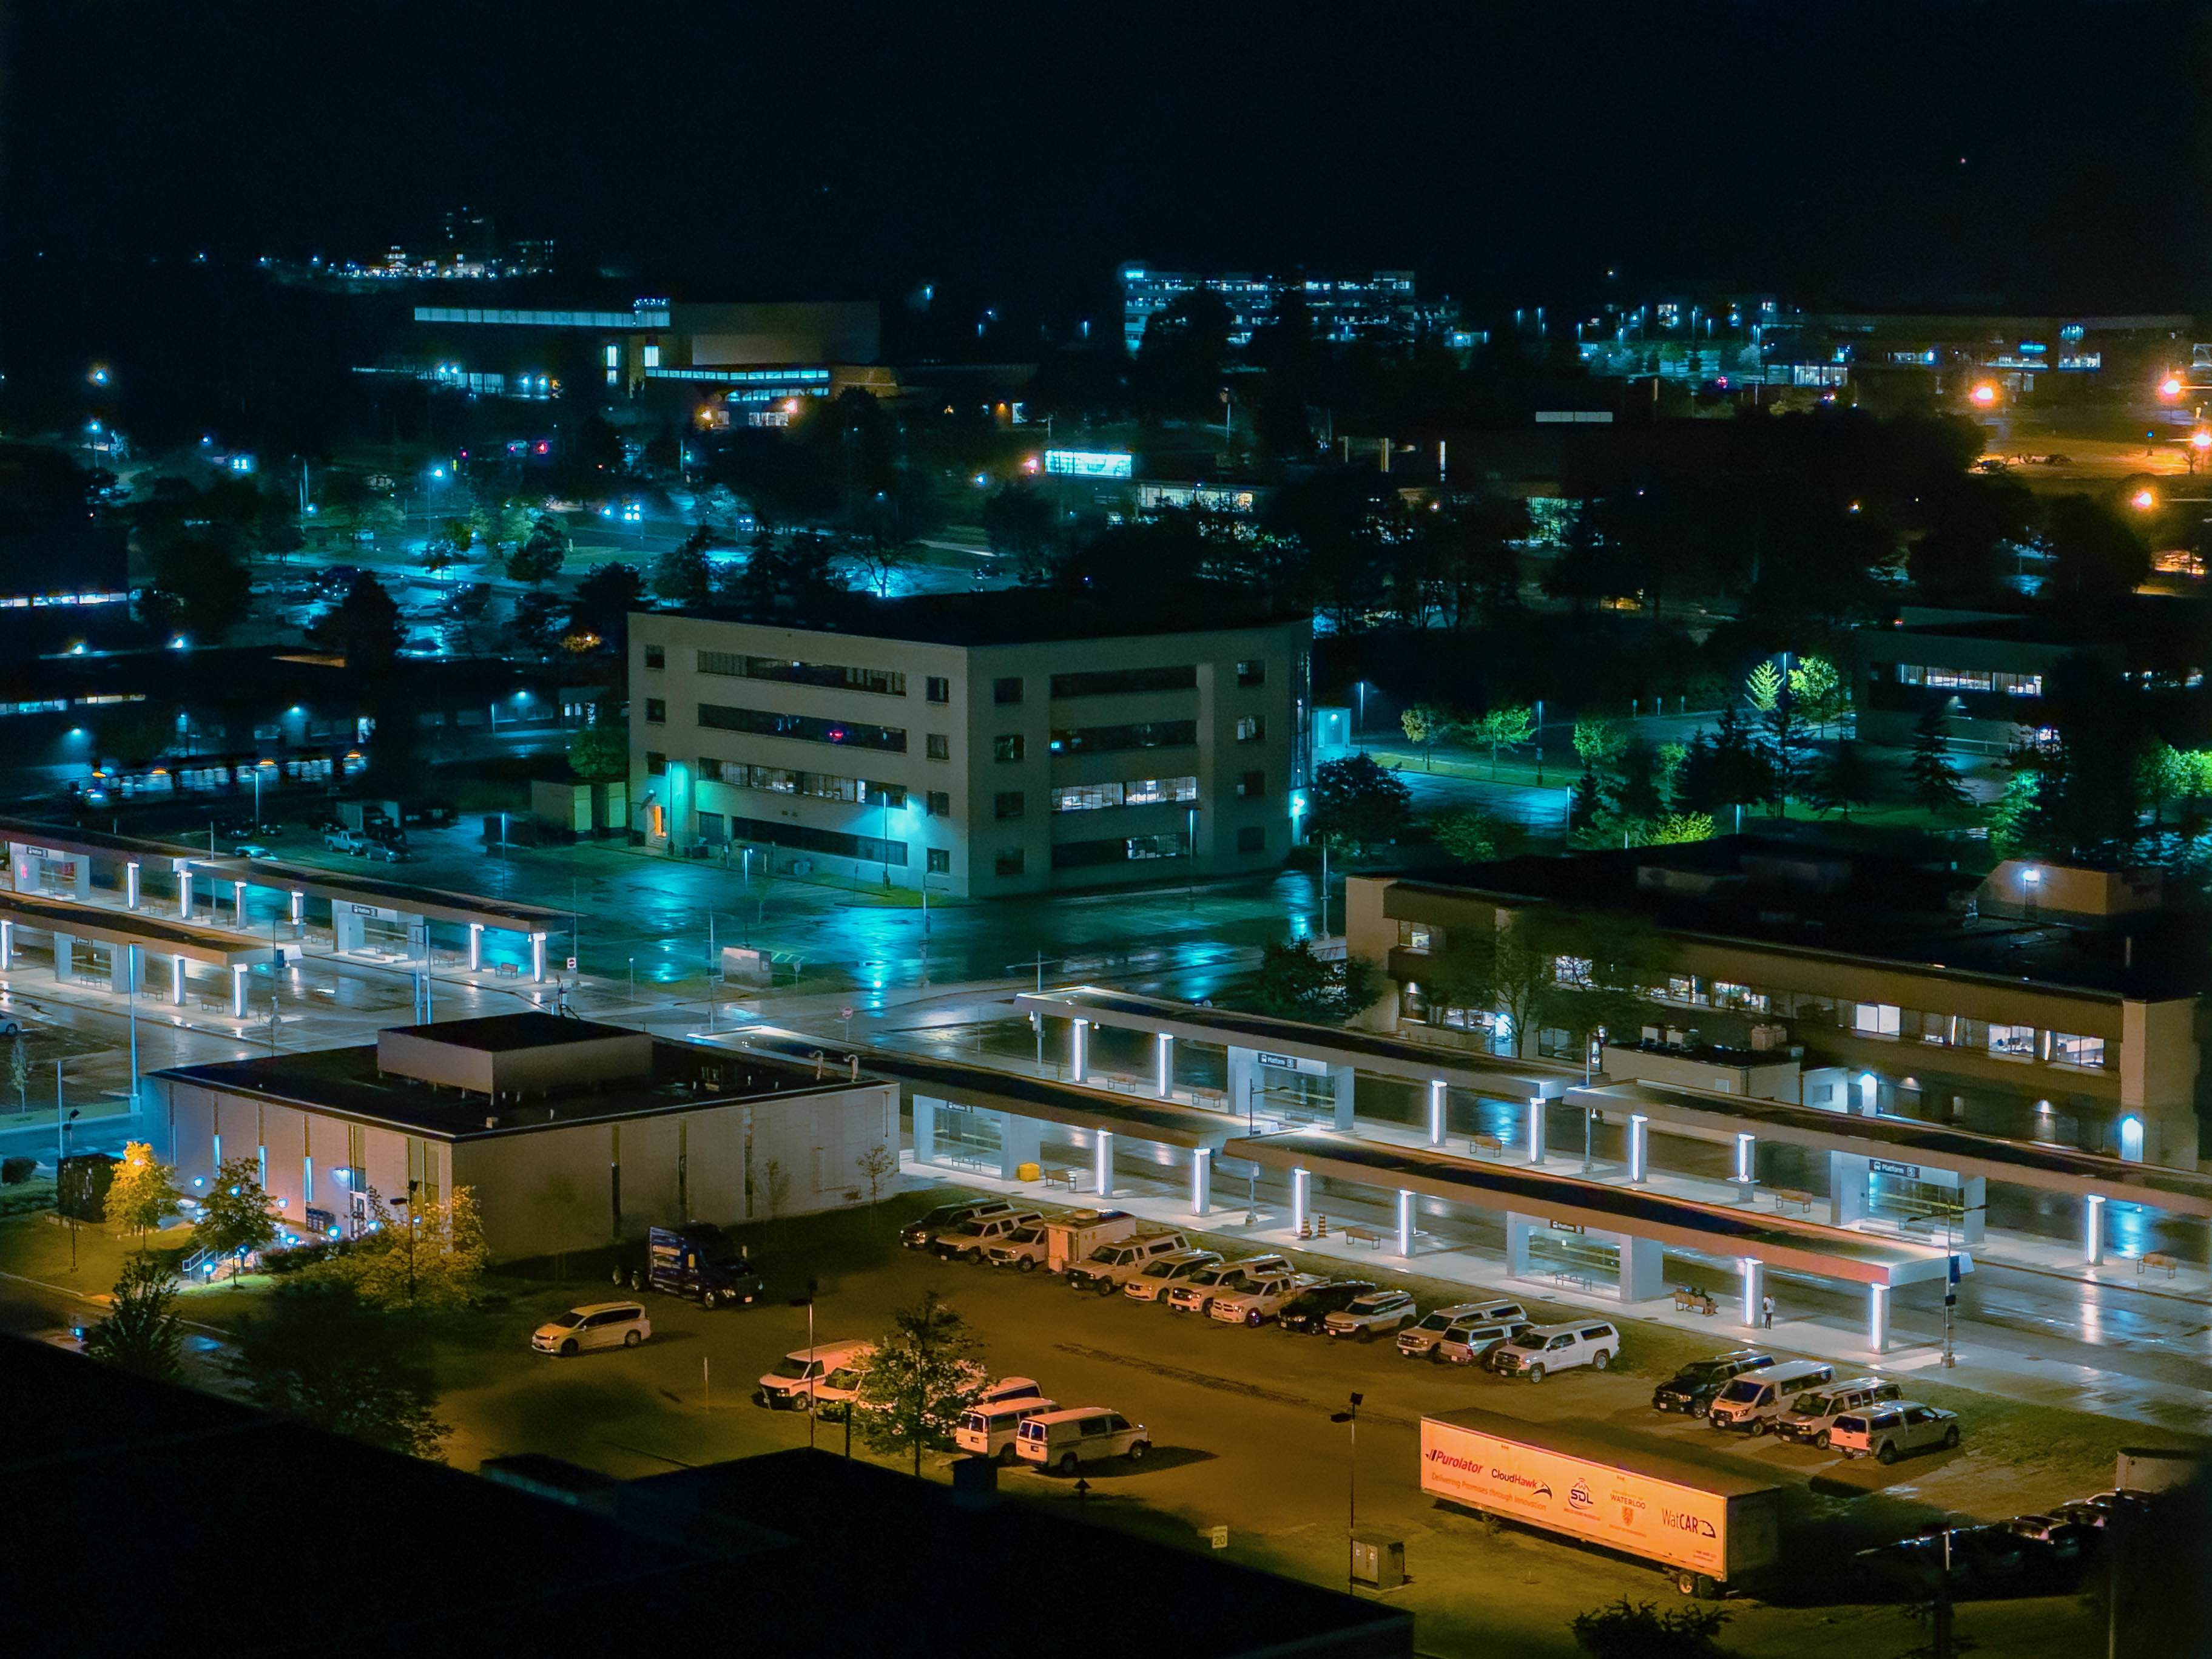
\includegraphics[scale=0.1]{img/loo.jpg}
%		\caption{Waterloo, ON}
%	\end{figure}
	
\end{document}
